% 9.(原油采购与加工)某公司用两种原油(A 和B)混合加工成两种汽油(甲和乙)。甲、乙两种汽油含原油A 的最低比例分别为50\%和60\%,每吨售价分别为4,800 元和5,600 元。该公司现有原油A 和B 的库存量分别为500 吨和1,000 吨,还可以从市场上买到不超过1,500 吨的原油A。原油A 的市场价为:购买量不超过500 吨时的单价为10,000 元/吨;购买量超过500吨但不超过1,000 吨时,超过500 吨的部分8,000 元/吨;购买量超过1,000 吨时,超过1,000 吨的部分6,000 元/吨。该公司应如何安排原油的采购和加工?请分别建立连续规划和整数规划模型来求解这个问题。

\subsubsection{问题分析}

该模型设计了一个生产场景,给出了两种原料的库存,原料采购的价格曲线,以及两种产品的成分约束以及市场价格,需要建立连续规划模型和整数规划模型。

\subsubsection{模型假设}

为了简化实际情况,模型基于以下假设,
\begin{enumerate}
    \item 混合过程中无物料损失,混合物能稳定共存。
    \item 原油采购是公司唯一的成本来源,汽油产品是唯一的收益来源。
    \item 汽油产品能在短时间内销售完毕。
\end{enumerate}

\subsubsection{模型建立}

\paragraph{连续规划} 设原油A中有$p$吨用于生产汽油甲,有$q$吨用于生产汽油乙,原油B中有$r$吨用于生产汽油甲,有$s$吨用于生产汽油乙,公司额外购买的原油A共$u$吨,购买总成本为$c$万元。则公司生产的汽油甲共$p+r$吨,乙共$q+s$吨。

汽油A,B需要满足的比例约束为,
\begin{equation}\label{eq:ex9_cons_prop}
    \frac{p}{p+r} \ge 50\%, \quad \frac{q}{q+s} \ge 60\%
\end{equation}

原油的总量约束为,
\begin{equation}\label{eq:ex9_cons_total}
    p+q \le 500 + u, \quad r+s \le 1000
\end{equation}

购买原油的总成本是关于购买量的分段函数,其图像如\Cref{fig:ex9_cost},数学表达式为,
\begin{equation}\label{eq:ex9_cons_seg}
    c = \begin{cases}
        u, & 0 \le u \le 500 \\
        0.8u + 100, & 500 < u \le 1000 \\
        0.6u + 300, & 1000 < u \le 1500
    \end{cases}
\end{equation}

还需要加上非负约束和取值范围约束,
\begin{equation}\label{eq:ex9_cons_range}
    p, q, r, s, u, c \ge 0, \quad u \le 1500
\end{equation}

需要最大化收益$f$,单位为万元,
\begin{equation}\label{eq:ex9_obj}
    \max f = 0.48(p+r) + 0.56(q+s) - c
\end{equation}

由于成本约束\Cref{eq:ex9_cons_seg}为非线性约束,因此这是一个非线性规划模型,决策变量为$p, q, r, s, u, c$,目标函数为\Cref{eq:ex9_obj},约束条件为\Cref{eq:ex9_cons_prop},\Cref{eq:ex9_cons_total},\Cref{eq:ex9_cons_seg}和\Cref{eq:ex9_cons_range}。

\paragraph{整数规划} 在连续规划的基础上,假设原油和汽油均为按吨买卖的,则需要增加整数约束,
\begin{equation}\label{eq:ex9_cons_int}
    p, q, r, s, u, c \in \mathbb{N}
\end{equation}

这就构成了一个整数规划模型,其决策变量为$p, q, r, s, u, c$,目标函数为\Cref{eq:ex9_obj},约束条件为\Cref{eq:ex9_cons_prop},\Cref{eq:ex9_cons_total},\Cref{eq:ex9_cons_seg},\Cref{eq:ex9_cons_range}和\Cref{eq:ex9_cons_int}。

\begin{figure}
    \centering
    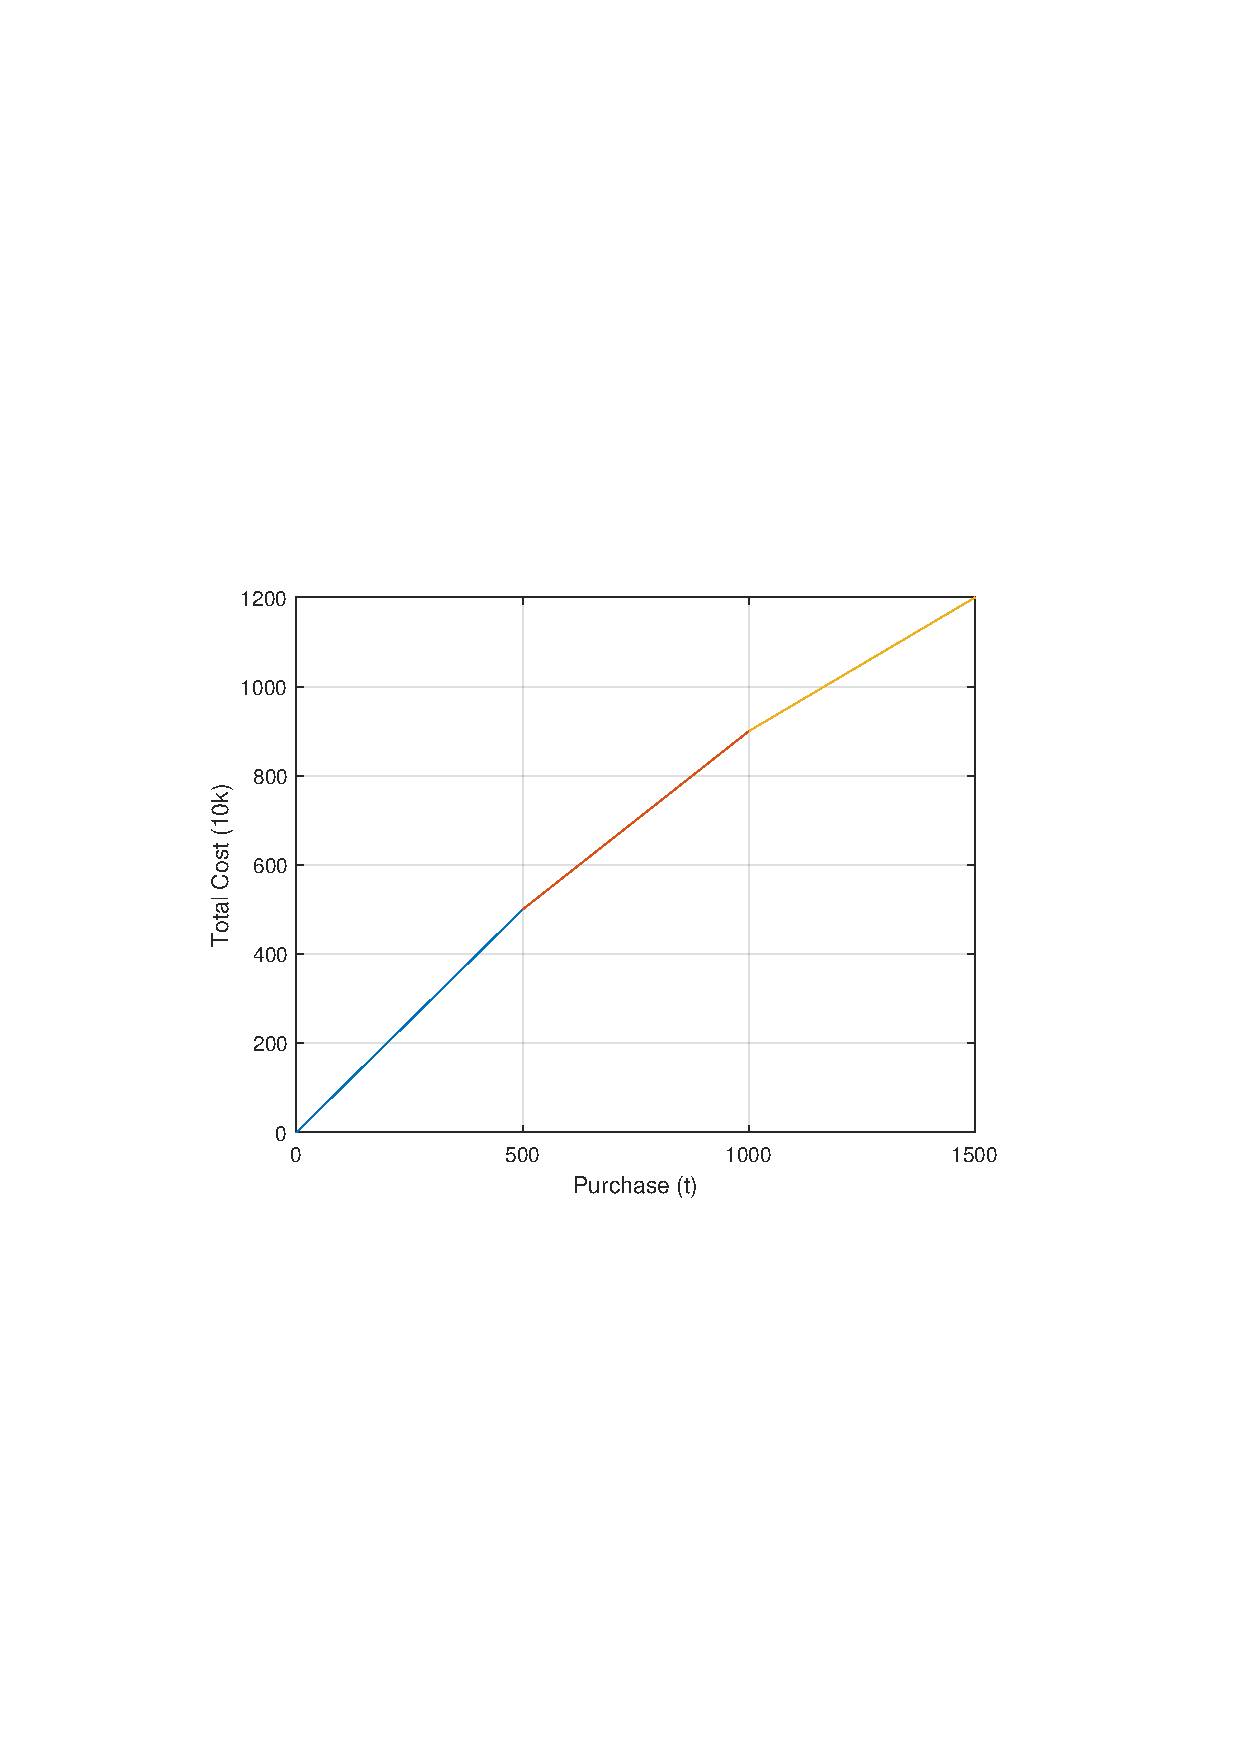
\includegraphics[width=0.8\textwidth,trim={3.09cm 9.295cm 3.09cm 9.295cm},clip]{fig/ex9_cost.pdf}
    \caption{总购买费用(万元)随购买量(吨)的变化图像}
    \label{fig:ex9_cost}
\end{figure}

\subsubsection{算法设计}

对于连续规划和整数规划,可使用LINGO软件求解,对于非线性约束\Cref{eq:ex9_cons_seg},可采用\texttt{@if}语句处理分段函数。

\subsubsection{程序}

请参见附录\ref{sec:ex9_code}。

\subsubsection{计算结果}

\paragraph{连续规划} LINGO将该问题识别为NLP (Nonlinear Program),经过19次迭代,求得全局最优解,得到总收益$f$的最大值为500万元,各决策变量的最优值为,
\begin{equation}
    p = 0, \quad q = 1500, \quad r = 0, \quad s = 1000, \quad u = 1000, \quad c = 900
\end{equation}

\paragraph{整数规划} LINGO将该问题识别为PINLP (Pure Integer Nonlinear Program),经过315次迭代,求得全局最优解,得到总收益$f$的最大值为500万元,各决策变量的最优值为,
\begin{equation}
    p = 0, \quad q = 1500, \quad r = 0, \quad s = 1000, \quad u = 1000, \quad c = 900
\end{equation}

\subsubsection{结果的数学分析}

连续规划模型与整数规划模型求出了相同的全局最优解,但在迭代次数上,整数规划是连续规划的17倍。

这启示我们,对于整数规划模型,可以先去掉整数约束,化为连续规划模型,如果求得的最优解恰好是整数解,那么这同样也是整数规划模型的最优解,但求解的时间复杂度从非多项式降低到了多项式;如果不是整数解,才需要进一步求解整数规划问题。

\subsubsection{结果的实际意义}

该计算结果具有一定的实际意义,可作为制定生产方案的重要参考。在实际应用中,还需要考虑原料供应量和产品需求量,原料和产品的价格波动等现实因素,根据实际情况对模型进行调整,才能做出切实可用的模型。

例如最近国际原油出现了破天荒的负油价,对应到模型中,就需要去掉原油价格的非负约束,受新冠疫情影响,未来的汽油消费预期并不乐观,对应到模型中,就需要考虑汽油产品的市场需求量,多余的产能是不能带来收益的。

\subsubsection{结论}

该公司应当花费900万元采购1000吨原油A,将所有1500吨原油A和1000吨原油B全部用来生产汽油乙,此时收益最高,为500万元。
